\paragraph{Firmware:} "Közvetlenül a hardvereszközzel egybeépített ROM, PROM vagy EPROM memóriamodulban tárolt szoftver,
amelynek feladata az eszköz működtetése, illetve az ahhoz szükséges alapvető be-/kimeneti rutinok biztosítása."\cite{tamas2019celzzott_firmware_def}
Ennek elemzése által az eszköz belső működéséről fontos információk nyerhetőek ki.
A szakdolgozat szempontjából releváns információak a következőek:
\begin{itemize}
    \item Nikon F parancs kódok
    \begin{itemize}
        \item Feladatuk
        \item Paramétereik
        \item Visszatérési értékeik
    \end{itemize}
    \item Nikon Z kamera objektívvezérlése
    \item Nikon FTZ adapter jelátalakítási eljárása
\end{itemize}
Egy ilyen adatkinyerési folyamat a következő lépásekből áll:
\begin{enumerate}
    \item Firmware beszerzése
    \item Firmware kicsomagolása
    \item Firmware Visszafordítása
\end{enumerate}\cite{nadir2022taxonomy}
\subsection{Firmware Beszerzése}
Három féle képpen lehet beszerezni egy eszközhöz a kapcsolódó firmware-t:
\begin{enumerate}
    \item Gyártótól való begyűjtés: Firmware letöltése a gyártó weboldaláról. \label{download_firmware_item}
    \item Hardverből történő kinyerés: Fizikai hozzáféréssel az eszközre már feltöltött kód kiolvasása.
    \item Vezeték nélküli frissítés során elfogás: A firmware "lefülelése" vezeték nélküli frissítés közben.
\end{enumerate} \cite{nadir2022taxonomy}
Nikon kamerákhoz, objektívekhez és egyéb kiegészítőkhöz a firmware frissítések online elérhetőek.
Ennek értelmében az \ref{download_firmware_item}-es számú módszer alkalmazható a firmware frissítésel rendelkező eszközökön.
Nikon kamera frissítésének folyamata a következő:
\begin{enumerate}
    \item Frissítés letöltése
    \item Frissítés kicsomagolása/kitömörítése \label{kicsomagolasi_lepes}
    \item Frissítés másolása kamera SD kártyára
    \item Kamera frissítése annak menüjéből
\end{enumerate}\cite{nikond5100_update_manual}
Itt a \ref{kicsomagolasi_lepes}-dik lépés után kapott fájllal folytatódik a folyamat.
Eddig a lépésig az objektívek/perifériák frissítésének lépései is megegyeznek, így azokon is ez a módszer alkalmazandó.
\subsection{Firmware kicsomagolása}
% the firmware is usually a binary file that encapsulates all the functionalities.
% The first step in reverse-engineering is the process of locating and extracting (and sometimes modifying and repacking) these functionalities from a single binary file. 
Az előző lépésben kapott bináris egy olyan fájl, amely tartalmaz minden funkcionalitást.
Ebben a lépésben ezek a funkcionalitások kerülnek szétbontásra, (és néha módosításra és újracsomagolásra).
Ide tartoznak a következő műveletek:
\begin{itemize}
    \item Titkosítás feloldása
    \item Fájlrendszer szétcsomagolása, fájlok elkülönítése
\end{itemize}\cite{nadir2022taxonomy}
A kamera firmware-en erre a műveletre elérhető eszköz a Nikon Patch\cite{Nikon_Patch}, amely elvégzi a binárison azon az obfuszkáció feloldását és a fájlrendszer felbontását is.
Ennek következtében a firmware ezen részén tovább vizsgálat szükségtelen.
Az eszköz azonban nem támogatja az objektíveket és a perifériákat, ezért azokon további műveletek elvégzése szükséges.
\subsubsection{Titkosítás/obfuszkáció felismerése entrópiavizsgálattal}
A firmware frissítések gyakran titkosítva/obfuszkálva vannak, ami nagyban megnehezíti azok elemzését.
Egy fájl titkosított/obfuszkált mivoltának mivoltára annak technika annak entrópiájának, tehát rendszertelenségének, vizsgálata.
A nagy entrópiájú, magas rendszertelenséggel rendelkező, fájlok nagy valószínűséggel titkosítottak/obfuszkáltak. \cite{miessler2015securing}
Egy linux eszközön a binwalk alkalmazás telepítés után egy bináris firmware fájlon a \textbf{\textit{binwalk -E\space [FÁJLNÉV]}} parancs használatával generálható le annak entrópiatérképe.
A Nikon FTZ adapter frissítésének \ref{kicsomagolasi_lepes}-es lépése után kapott fájlon az elemzést elvégezve az alábbi eredmény kapható:
\begin{figure}[H]
	\centering
	\includegraphics[width=0.7\linewidth]{img/Nikon_FTZ_entrópia.png}
	\caption{Nikon FTZ adapter firmware entrópiája}
	\label{fig:Nikon_FTZ_entrópia}
\end{figure}
Az analízis alapján belátható, hogy a fájl valamilyen módon titkosítva/obfuszkálva van, mivel az entrópiája konstans és magas.
Ezzel szemben a Nikon D5100 firmware entrópiája a következőképpen alakul az obfuszkáció feloldásával:
\begin{figure}[H]
	\centering
	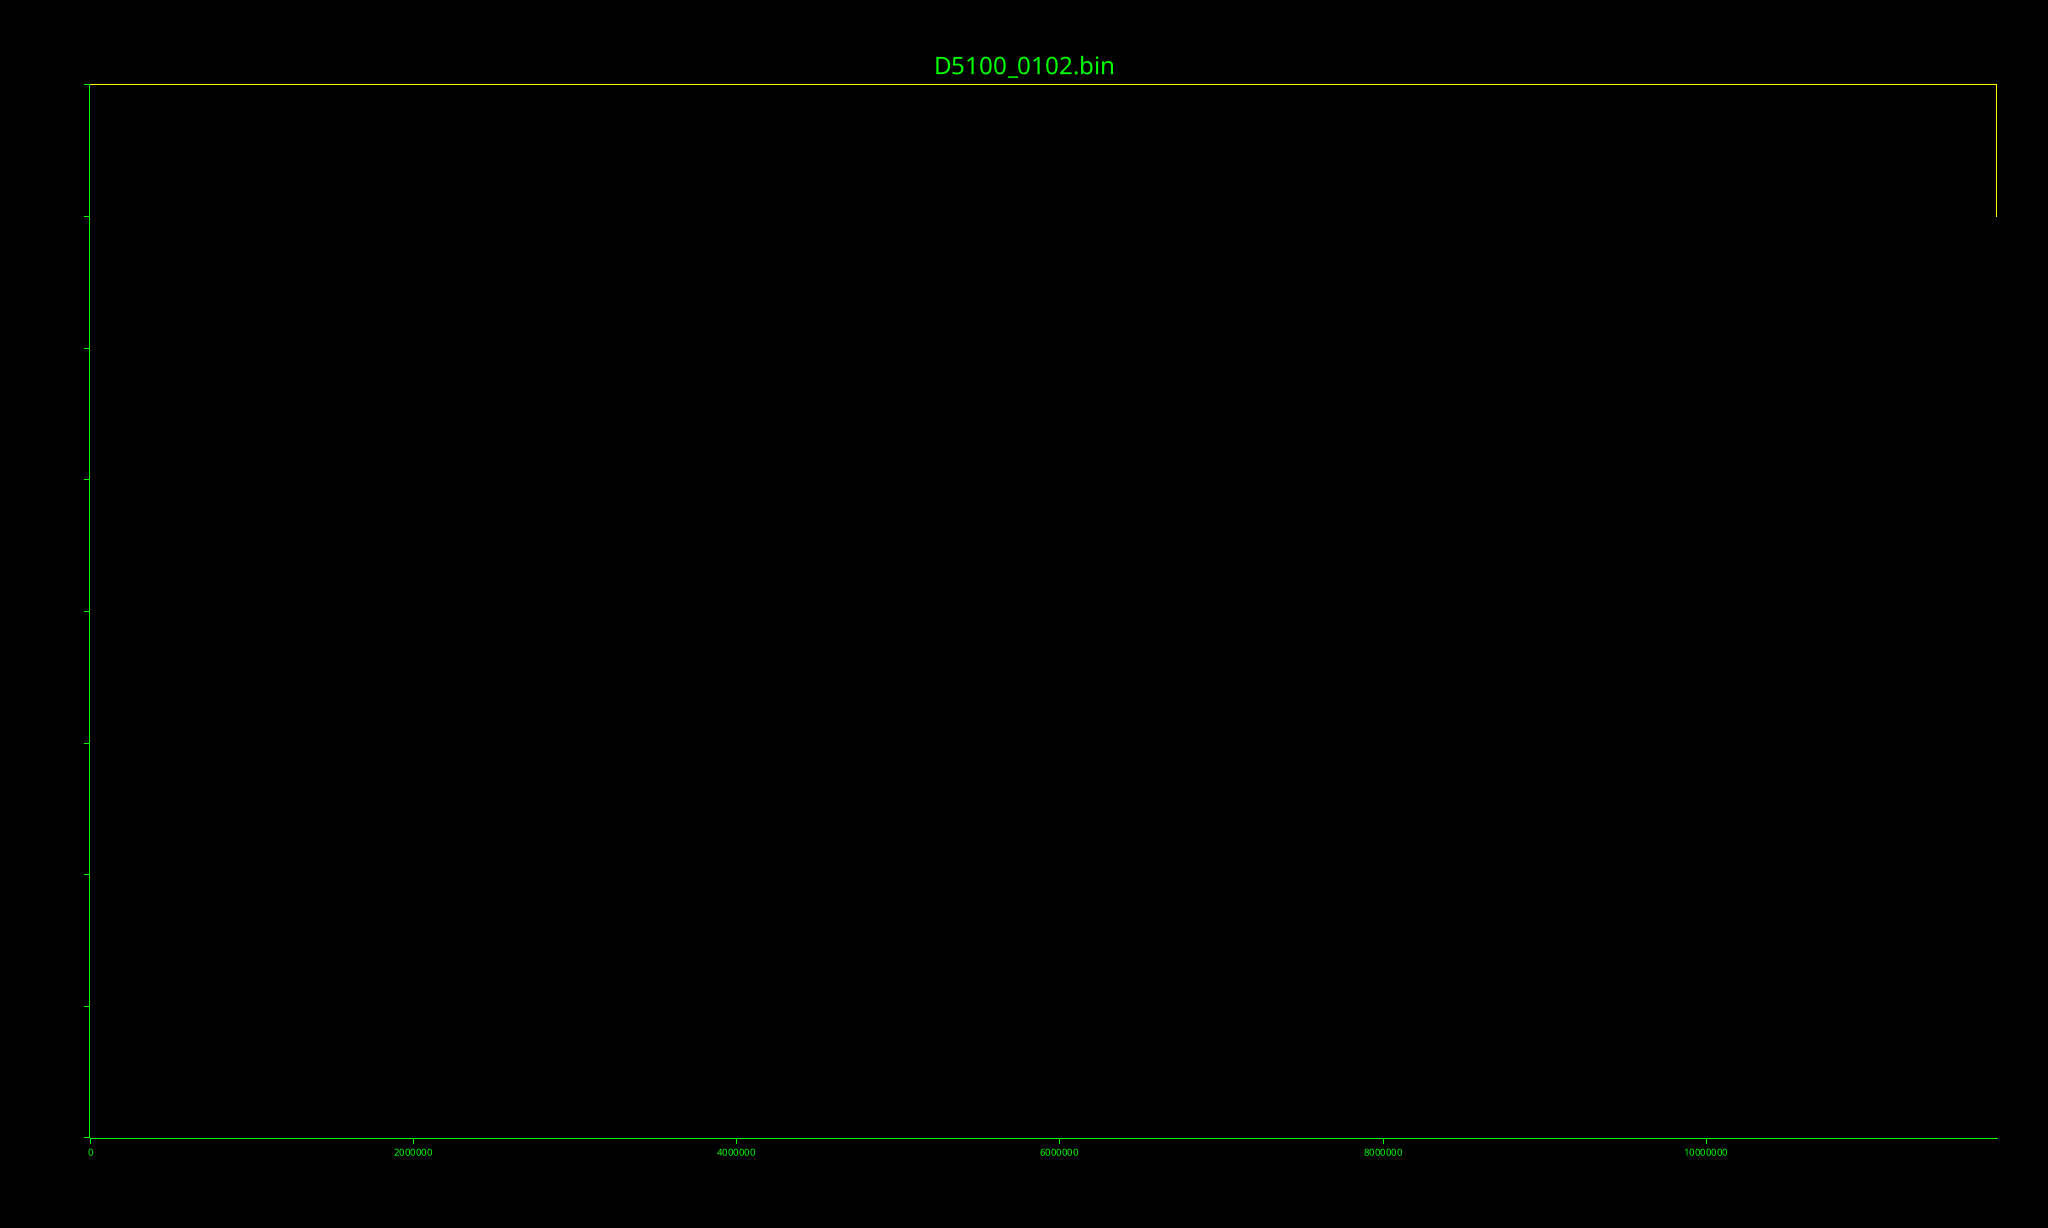
\includegraphics[width=0.7\linewidth]{img/D5100_before.png}
	\caption{Nikon D5100 firmware entrópiája obfuszkációval}
	\label{fig:Nikon_5100_elotte_entropia}
\end{figure}\begin{figure}[H]
	\centering
	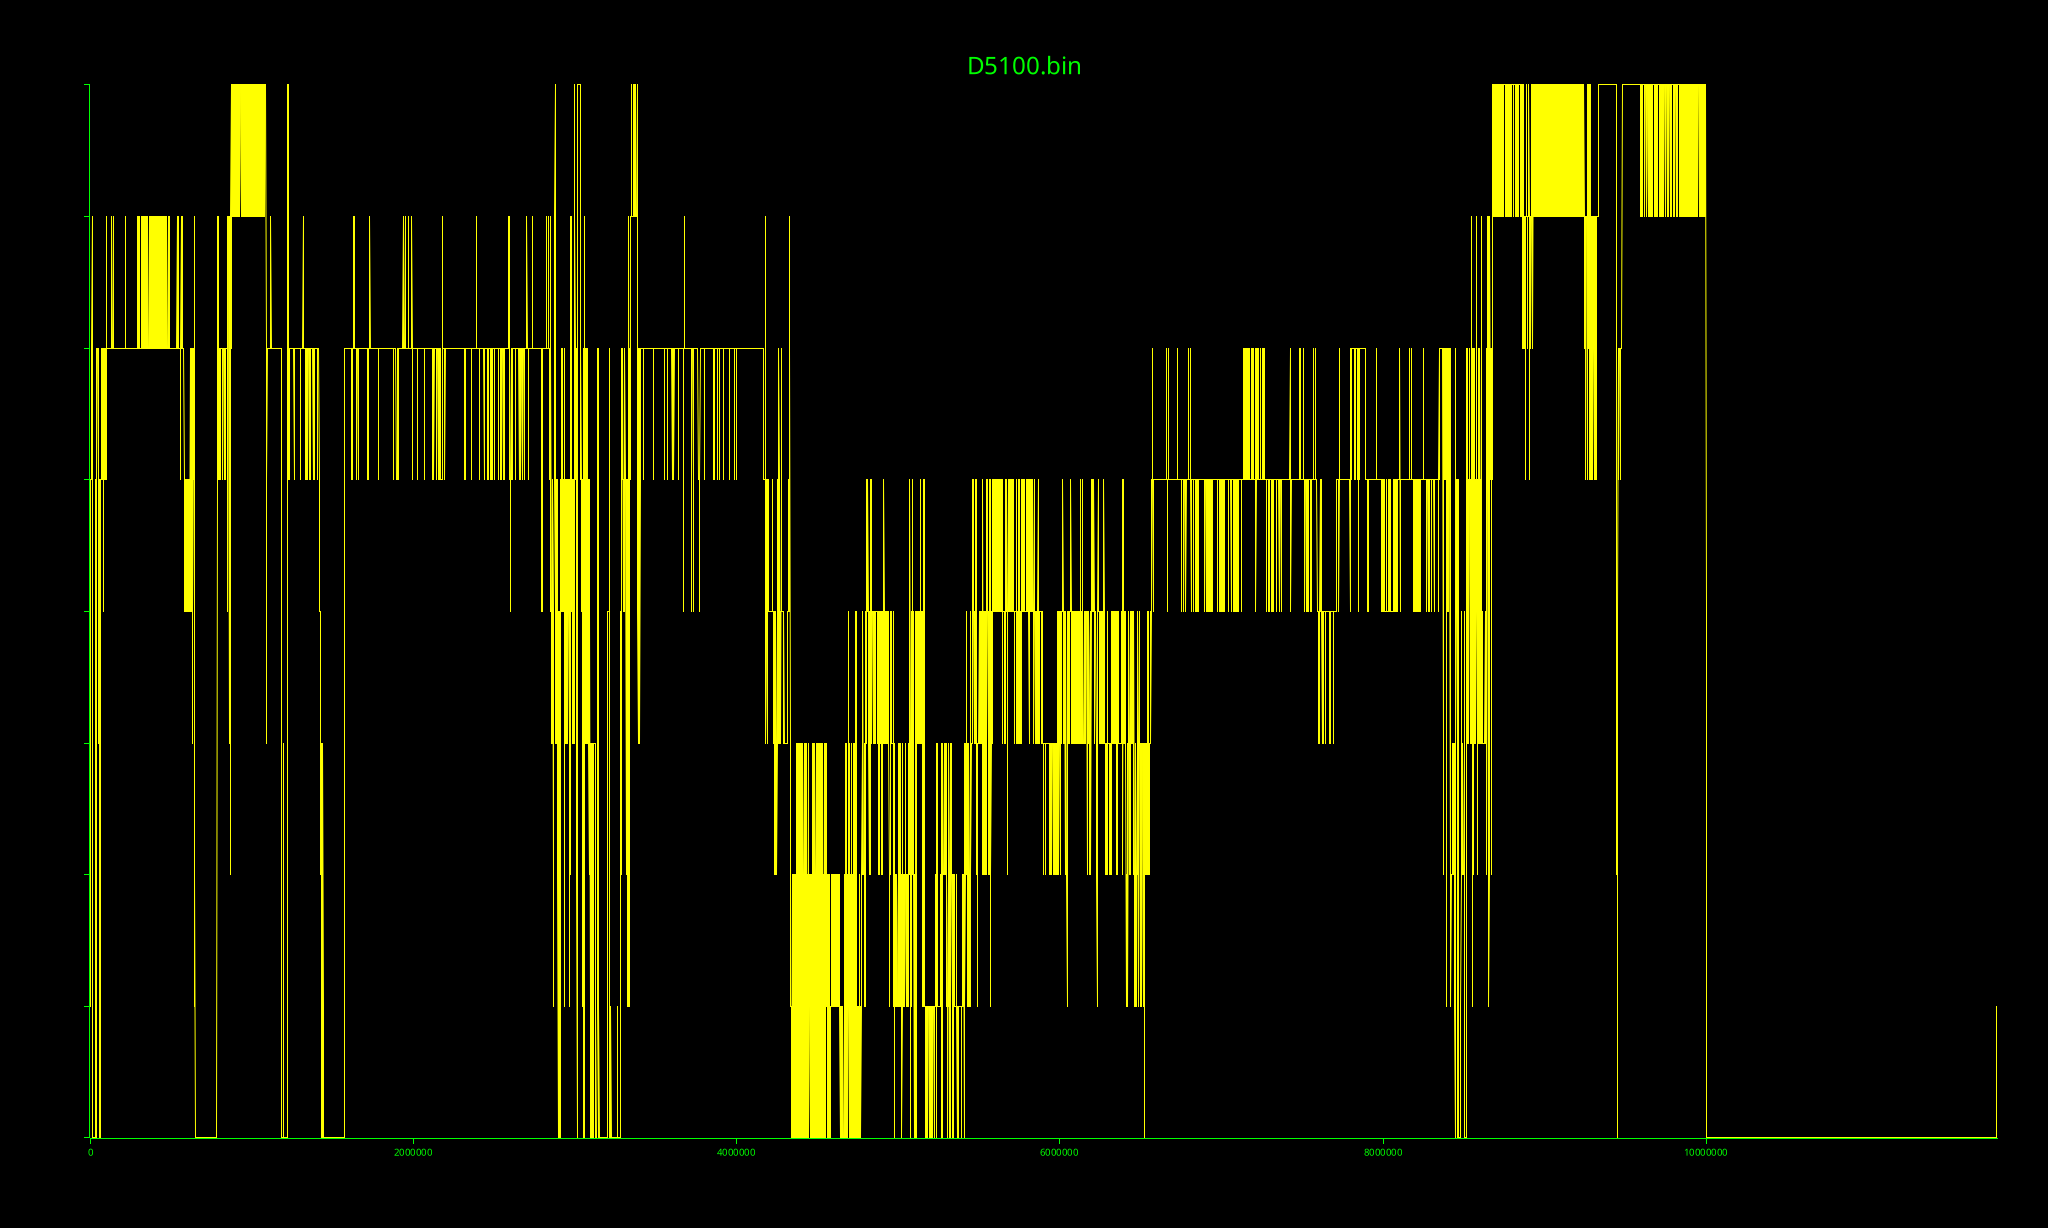
\includegraphics[width=0.7\linewidth]{img/D5100_after.png}
	\caption{Nikon D5100 firmware entrópiája obfuszkáció nélkül}
	\label{fig:Nikon_5100_utana_entropia}
\end{figure}
Ebben az esetben látható, hogy az obfuszkáció eltávolítása után az entrópia csökkent, és változatosabbá vált.

Mivel a szakdolgozatnak nem célja titkosítások/obfuszkációk feltöréséhez eszközt fejleszteni, ezért a perifériák, beleértve a Nikon FTZ adpater, firmware-jeinek vizsgálata ezzel lezárul.
\subsubsection{Kamera firmware}
A Nikon DSLR kamerák 2 különböző firmware-el rendelkeznek, amik a kamerák jól elkülöníthető funkcióikért felelnek.
A Nikon ezeket A és B firmware-nek hívja\cite{nikon_support_firmware_list}.
Ezekből a szakdolgozathoz az A firmware tartalmazhat hasznosítható információt,
mivel az felelsős az ki/bemeneti műveletekért, aminek a részét képzi az objektívekkel történő kommunikáció is\cite{nikonhackers_understanding_firmware}.

\subsection{Firmware Visszafordítása}
Ennek a fázisnak célja az, hogy protokollkódok, kommunikációs rutinok és más hasonló elemek kinyerése.
Az eredmények segítenek megérteni a működést elektronikus jelek eltérítése, elfogása nélkül.
\subsection{Disassembálás}
"A gépi kódú bájtok ember által olvasható assembly utasításokká történő visszafejtése."\cite{zhang2024disassembling}

Hátránya a kifelyezetten ISA specifikus, nagyon nehezen olvasható kód, amelyhez szükséges az architektúra részletes ismerete.
Mivel a program obfuszkált, ezért az eredeti kód szimbólumai el lettek belőle távolítva, ezért az ennél a lépésnél kapott assembly kód sem tartalmazza azokat.
Ennek következtében a kód értelmezése még nehezebbé válik, és önmagában akár felfedhetetlen is marad.

A Nikon Emulator segítségével az A firmware disassemblálható, viszont nem visszaforditható.
A legnagyobb támogatással a D5100 firmware-je rendelkezik. Ez a MIPS16 ISA-nak egy kiegészített változatával rendelkező processzorokon való futtatásra lett készítve.\cite{nikonhackers_understanding_firmware}
Emiatt at így kapott assembly is TX19A-lesz.
Ennek az olvasása az eltávolított szimbólumok mellett még úgy is nehézkes, hogy a disasszembláló a diszasszemblált D5100 firmware-hez korábbi megfigyelések alapján egyéni szimbólumokat is beépít.
Ezért az assembly visszafordítása szükséges egy magasabb szintű nyelvre mint például a C.

\subsection{Visszafordító eszközök}
A disassemblálás során kapott assembly kód továbbra is nehezen értelmezhető, és nagy valószínűséggel a program sem ebben íródott.
Arra, hogy a kód még olvashatóbb legyen, program visszafórdító alkalmazandó, amely jóval egyszerűbben olvashatóbb és értelmezhetőbb C nyelvű kódot eredményez. 

\subsubsection{Ghidra}
Az Egyesül Államok Nemzetbiztonsági Ügynöksége (NSA) által fejlesztett szabad forráskódú visszafordító eszköz.
Nagyban módosítható és bővíthető, széleskörű ISA támogatással.
A saját területspecifikus programozási nyelvével egyedi ISA-kkal is bővíthető.
A dekompilált/visszafordított kód jó minőségű.
Hátránya nehezen használható felhasználói felület.

\subsubsection{IDA}
Az IDA az első visszafordító alkalmazás volt, és a mai napig megtartotta a relevanciáját a jó visszafordítási eredményei miatt.
Zárt forráskódú fizetős szoftver, amiből ingyenes verzió is elérhető kizárólag x86-os architektúra támogatással.
Az egyéb architektúrák eléréséhez elő kell fizetni egy szoftver liszenszre.
Az árazás 330\texteuro/év-től kezdődik, amely a dolgozat költségvetése felett van.

\subsubsection{Eredmény}
\paragraph{Ghidra}
Nem támogatja a TX19A ISA-t, azonban a MIPS16-ra alapozva lehet írni hozzá kiegészítést, amely hozzáadja a támogatást, ez azonban a dolgozat korlátain túl mutat.
\paragraph{IDA}
MIPS16-támogatással rendelkező szoftverliszensz esetén hozzáadható egy olyan plugin, amely hozzáadja a TX19A támogatást
Mivel a pénzügyi kereten ez túlmutatja, ezért nem lehet vele visszafordítani a programot.

\paragraph{Konklúzió}A visszafordítási fázis sikertelen volt.


